%!TEX root = karen.tex


\chapter{The RBF-generated Finite Differences Method}

The process of solving PDEs using RBFs dates back to 1990 \cite{Kansa1990a,Kansa1990b}. This chapter starts with a description of the general approximation problem and provides background on RBF scattered data interpolation that will be required for the remainder of the chapter. This is followed by a description of Radial Basis Function-generated Finite Differences and examples of operators approximated by the method within this work.

We categorize existing methods for solving PDEs with RBFs as either global or local. Global methods use collocation and invert a single large linear system to find the interpolant that satisfies the differential equations at nodes in the domain. Local methods limit the influence of basis functions and seek an interpolant at each node defined in terms of neighboring basis functions (local collocation) or nodal values (RBF-FD). \authnote{list references of each type} \authnote{Do I need to define global collocation in the dissertation? The only purpose would be to compare complexity of RBF-FD with it}

\section{Background}

Consider a PDE expressed in terms of (linear) differential operators, $\diffop$ and $\boundop{}$: 
\begin{eqnarray}
\diffop{u} & = & f \on{\Interior}, \nonumber \\
\boundop{u} &=& g \on{\Boundary} 
\end{eqnarray}
where $\Interior$ is the interior of the physical domain, $\Boundary$ is the boundary of $\Interior$ and $f,g$ are known explicitly. In the case of a non-linear differential operator, a Newton's iteration, or some other method, can be used to linearize the problem (see e.g., \cite{WrightFornberg06}); of course, this increases the complexity of a single time step. 

We solve PDEs of this form with \emph{collocation}. That is, given a number of points in the domain, derivative and solution values are sought to best satisfy $f, g$ at node locations. \authnote{Not clear yet. Review Lynch2005 for a better explanation}\cite{Lynch2005}

\section{Stencil-based Derivative Approximation}

The RBF-FD method is similar to classical Finite Differences in that differential quantities at a single node referred to as a \emph{center}, $\vx_{j}$, is approximated by weighted combinations of function values at $n-1$ neighboring nodes. The center node and its neighbors define a \emph{stencil}, $\{\vx\}_{i=1}^{n}$, in a localized (small) region or \emph{neighborhood} of the domain. 


We define a \emph{stencil} is generated connecting the center node and its nearest neighbors.  Figure~\ref{fig:stencil_example} provides two examples of stencils. First, Figure~\ref{fig:stencil_example_random} illustrates a single stencil of size $n=13$ in a domain of randomly distributed nodes. The stencil center is represented by a green square, with the 12 neighboring nodes connected via red edges. The purple circle, the minimum covering circle for the stencil, demonstrates that the stencil contains only the 12 nearest neighbors of the center node. In Figure~\ref{fig:stencil_example_sphere}, a larger RBF-FD stencil of size $n=75$ on the unit sphere is shown as red and blue disks surrounding the center represented as a square. Green disks are nodes outside of the stencil. The radii and color the red and blue disks represent the magnitude and sign of the RBF-FD weights determined to calculate a derivative quantity at the stencil center. 

\begin{figure}[htbp]
	\centering
	\begin{subfigure}[m]{0.35\textwidth}
		\centering
		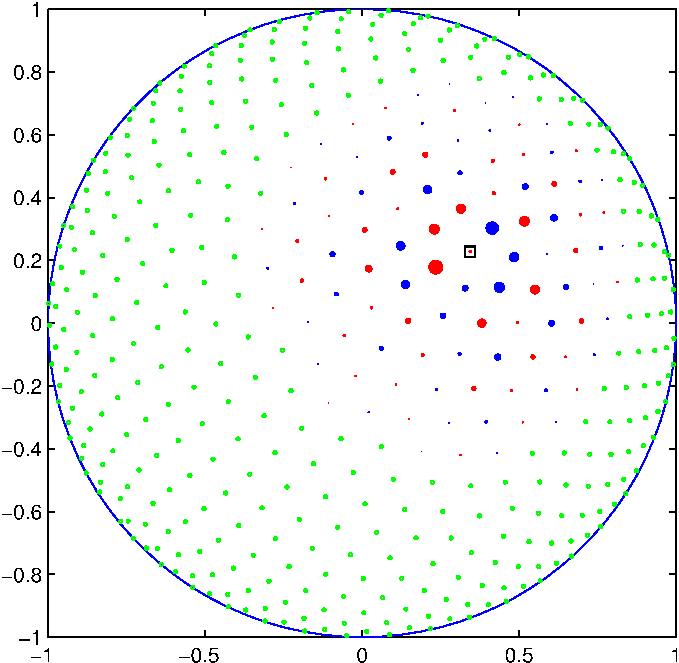
\includegraphics[width=1.0\textwidth]{figures/chapter1/RBFFD_single-eps-converted-to.pdf}
		\caption{A 75 node RBF-FD stencil with blue (negative) and red (positive) differentiation weights to approximate advective operator at the square. Stencils weights indicated by scale of disk radii. (Image courtesy of Bengt Fornberg and Natasha Flyer)}
		\label{fig:stencil_example_sphere}
	\end{subfigure}
	\begin{subfigure}[m]{0.6\textwidth}
		\centering
		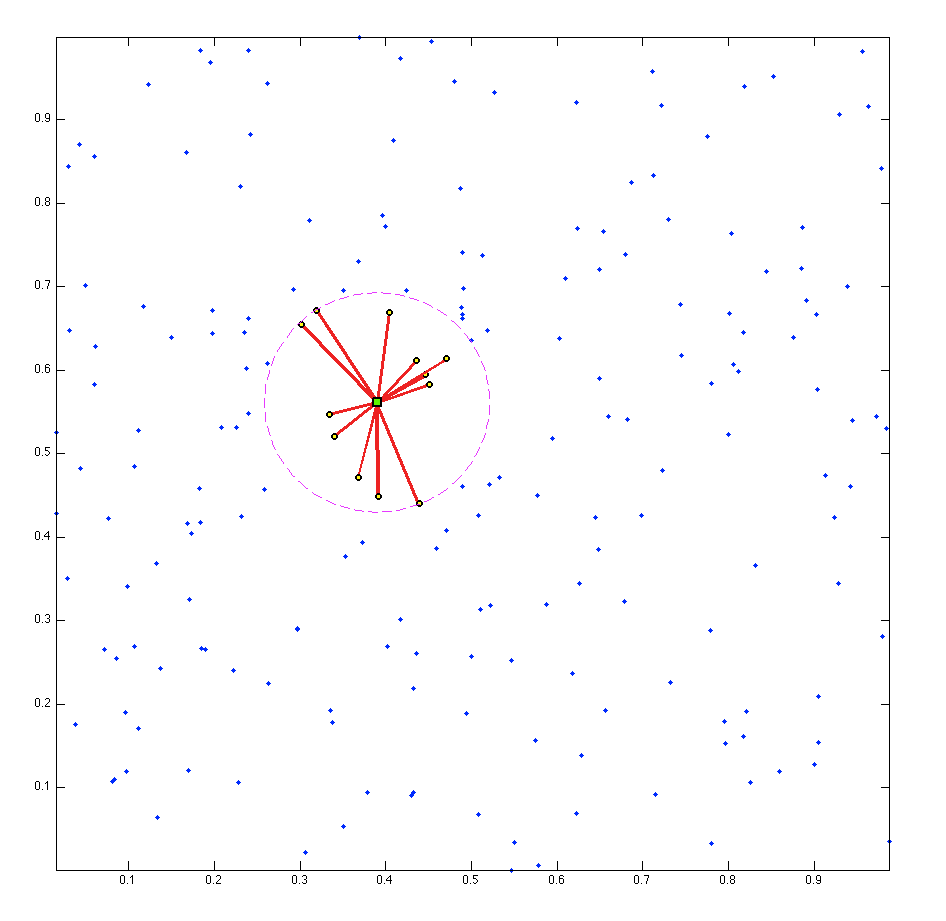
\includegraphics[width=1.0\textwidth]{figures/chapter1/preview_stencils_example.png}
		\caption{A 13 node RBF-FD stencil of randomly distributed nodes. The stencil centered at the green square contains the 12 nearest neighbors contained within the minimum covering circle drawn in purple.}
		\label{fig:stencil_example_random}
	\end{subfigure}
	\caption{Examples of stencils computable with RBF-FD \authnote{Consider: show example FD stencil (5pt with regular grid)}}
	\label{fig:stencil_example}
\end{figure}


\section{RBF-FD weights}
\label{sec:rbffd}

Given a set of function values, $\{u(\vx_j)\}_{j=1}^{N}$, on a set of $N$ nodes $\{\vx_j\}_{j=1}^{N}$, the operator $\diffop$ acting on $u(\vx)$ evaluated at 
$\vx_j$, %$u(\vx_j)$ 
is approximated by a weighted combination of function values, $\{u(\vx_i)\}_{i=1}^{n}$, in a small neighborhood of $\vx_j$, 
where $n\ll N$ defines the size of the stencil. 
%(added constant term to equation:)
\begin{align}
\diffop{u(\vx)}\mid_{\vx=\vx_j} &\approx \sum_{i=1}^{n} w_i u(\vx_i) + w_{n+1} p_0
\label{eq:derivFromFDWeights}
\end{align}
The RBF-FD weights, ${w_i}$, are found by enforcing that they are exact within the space spanned by the RBFs $\phi_i(\epsilon r) = \phi(\ep\vectornorm{\vx-\vx_{i}})$, centered at the nodes $\{\vx_i\}_{i=1}^{n}$, with 
$r=\vectornorm{\vx - \vx_i}$
being the distance between where the RBF is centered and where it is evaluated as measured in the standard Euclidean 2-norm. Various studies show  \cite{WrightFornberg06,FornbergDriscoll02,FornbergLehto11,FlyerLehto11} that better accuracy is achieved when the 
interpolant can exactly reproduce a constant, $p_0$.  
Assuming $p_0 = 1$, the constraint $\sum_{i=1}^{n}w_i=\diffop{1}|_{\vx=\vx_{j}}=0$ completes the system: 
%Address how the constraint is added. $w_{n+1}$ is mentioned without being defined.
%($\epsilon$ has been moved outside the norm on the RHS)
\begin{align}
\begin{pmatrix}
\phi(\epsilon\vectornorm{\vx_1-\vx_1}) & \phi(\epsilon\vectornorm{\vx_1-\vx_2} & \cdots & \phi(\epsilon\vectornorm{\vx_1-\vx_n}) & 1 \\
\phi(\epsilon\vectornorm{\vx_2-\vx_1}) & \phi(\epsilon\vectornorm{\vx_2-\vx_2} & \cdots &
\phi(\epsilon\vectornorm{\vx_2-\vx_n}) & 1\\
\vdots & \ddots & \ddots & \vdots & \vdots\\
\phi(\epsilon\vectornorm{\vx_n-\vx_1}) & \phi(\epsilon\vectornorm{\vx_n-\vx_2} & \cdots &
\phi(\epsilon\vectornorm{\vx_n-\vx_n}) & 1 \\
1 & 1 & \cdots & 1 & 0
\end{pmatrix}
\begin{bmatrix} w_1 \\ w_2 \\ \vdots \\ w_n  \\ w_{n+1}\end{bmatrix}
&=
\begin{bmatrix} \diffop{\phi(\ep\vectornorm{\vx-\vx_{1}})}|_{\vx=\vx_{j}} \\
                \diffop{\phi(\ep\vectornorm{\vx-\vx_{2}})}|_{\vx=\vx_{j}} \\ \vdots \\  \diffop{\phi(\ep\vectornorm{\vx-\vx_{n}})}|_{\vx=\vx_{j}}\\
                0
\end{bmatrix},
\label{eq:rbffd_weight_system}
\end{align}
where $w_{n+1}$ is ignored after the matrix in ({\ref{eq:rbffd_weight_system}}) is inverted.
This $n \times n$ system solve is repeated for each stencil center  $\vx_j$, $j=1...N$, to form the $N$ rows of the DM  with $n$ non-zeros $(n\ll N)$ per row.
As an example, if $\diffop$ is the identity operator, 
then the above procedure leads to RBF-FD interpolation. If $\diffop=\pd{}{x}$, one obtains the DM that approximates the first derivative in $x$. In the context of time-dependent PDEs,  the stencil weights remain constant for all time-steps when the nodes are stationary. Therefore, the calculation of the 
differentiation weights is performed once in a single preprocessing step of O$(n^3N)$ 
%floating point operations (FLOPs). 
FLOPs.
Improved efficiency is achieved
by processing multiple right hand sides in one pass, calculating the weights
corresponding to all required derivative quantities (i.e., $\pd{}{x}$, $\pd{}{y}$, $\Laplacian$, etc.).

%reply to the LSH question from the reviewer involving parallelization of the search process for each point, and the issue regarding embarrassingly parallel process. Also note: this is done only once so efficiency is not an issue, nor is parallelization.

For each of the $N$ small system solves of Equation~(\ref{eq:rbffd_weight_system}), the $n$ nearest neighbors to $\vx_j$ need to be located. This can be done efficiently using neighbor query algorithms or spatial partitioning data-structures such as Locality Sensitive Hashing (LSH) and $k$D-Tree. Different query algorithms often have a profound impact on the DM structure and memory access patterns. We choose a Raster ($ijk$) ordering LSH algorithm \cite{Bollig2011} leading to the matrix structure in Figures~\ref{fig:oneThreadPerStencil} and \ref{fig:oneWarpPerStencil}. While querying neighbors for each stencil is an embarrassingly parallel operation, the node sets used here are stationary and require stencil generation only once. Efficiency and parallelism for this task has little impact on the overall run-time of tests, which is dominated by the time-stepping. We preprocess node sets and generate stencils serially, then load stencils and nodes from disk at run-time. In contrast to the RBF-FD view of a static grid, Lagrangian/particle based PDE algorithms promote efficient parallel variants of LSH in order to accelerate querying neighbors at each time-step \cite{Pan2011, Goswami2010}. 


\section{Weight Operators}
Throughout the development of our parallel code we have verified code correctness through the solution of a variety of PDEs. Here we provide a list of operators we have tested and their corresponding equations for the RHS of Equation~\ref{eq:rbffd_weight_system} necessary to compute RBF-FD weights. 

The standard first derivatives $\pd{}{x}, \pd{}{y}, \pd{}{z}$:
\begin{itemize}
	\item $\pd{\phi}{x}  $
\end{itemize} 

where $\pd{\phi}{r}$ for the Gaussian RBFs is given by: 


\subsection{Laplacian ($\Laplacian$)}

2D: 

3D: 

\subsection{Laplace-Beltrami ($\LaplaceBeltrami$) on the Sphere}

The $\Laplacian$ operator can be represented in spherical polar coordinates for $\mathbb{R}^3$ as: 
\begin{align} 
\Laplacian = \underbrace{\frac{1}{r} \pd{}{r} \left( r^{2} \pd{}{r}  \right)}_{\mathsf{radial}} + \underbrace{\frac{1}{r^2} \Delta_{S}}_{\mathsf{angular}} , \label{eq:laplacian_in_spherical}
\end{align}
where $\LaplaceBeltrami$ is the Laplace-Beltrami operator---i.e., the Laplacian operator constrained to the surface of the sphere. This form nicely illustrates the separation of components into radial and angular terms. 

In the case of PDEs solved on the unit sphere, there is no radial term, so we have:
\begin{align}
\Laplacian  \equiv \LaplaceBeltrami.
\end{align}
Although this originated in the spherical coordinate system, \cite{WrightFlyerYuen10} introduced the following Laplaci-Beltrami operator for the surface of the sphere: 
\begin{align} 
\LaplaceBeltrami = \frac{1}{4} \left[ \left(4-r^2\right) \pdd{}{r} + \frac{4-3r^2}{r} \pd{}{r} \right],
\end{align} 
where $r$ is the Euclidean distance between nodes of an RBF-FD stencil and is independent of our choice of coordinate system. 

\subsection{Constrained Gradient ($P_{x} \cdot \grad$) on the Sphere}

Additionally following \cite{FlyerWright09, FlyerLehto11}, the gradient operator must also be constrained to the sphere with this projection matrix: 
%\frac{1}{||\mathbf{x}||}
\begin{align}
P = I - \mathbf{x} \mathbf{x}^T =  \begin{pmatrix} 
(1-x_1^2) & -x_1 x_2 & -x_1 x_3 \\
-x_1 x_2 & (1-x_2^2) & -x_2 x_3 \\ 
-x_1 x_3 & -x_2 x_3 & (1-x_3^2) 
\end{pmatrix} = \begin{pmatrix} P_{x_1} \\ P_{x_2} \\ P_{x_3} \end{pmatrix}
\label{eq:project_gradient}
\end{align}
where $\mathbf{x}$ is the unit normal at the stencil center. 


The direct method of computing RBF-FD weights for the projected gradient for $\mathbf{P} \cdot \nabla $ is presented in \cite{FlyerWright09}. When solving for the weights, we apply the projection on the right hand side of our small linear system. We let $\vx = \begin{pmatrix} x_1, x_2, x_3 \end{pmatrix} $ be the stencil center, and $\vx_k=\begin{pmatrix} x_{1,k}, x_{2,k}, x_{3,k}\end{pmatrix}$ indicate an RBF-FD stencil node. 

Using the chain rule, and assumption that 
$$r(\vx_k-\vx)=\vectornorm{\vx_k-\vx} = \sqrt{(x_{1,k}-x_1)^2 + (x_{2,k}-x_2)^2 + (x_{3,k}-x_3)^2},$$
 we obtain the unprojected gradient of $\phi$ as
$$\nabla \phi(r(\vx_k - \vx)) = \pd{r}{\vx} \pd{\phi(r(\vx_k - \vx))}{r} = - (\vx_k - \vx)\frac{1}{r(\vx_k - \vx)} \pd{\phi(r(\vx_k - \vx))}{r}$$. 

Applying the projection matrix gives 
\begin{align*}
\mathbf{P} \nabla \phi(r(\vx_k - \vx)) & = - (\mathbf{P} \cdot \vx_k - \mathbf{P}\cdot\vx)\frac{1}{r(\vx_k - \vx)} \pd{\phi(r(\vx_k - \vx))}{r} \\
& =  - (\mathbf{P}\cdot\vx_k - 0)\frac{1}{r(\vx_k - \vx)} \pd{\phi(r(\vx_k - \vx))}{r} \\
& = - (I-\vx\vx^T)(\vx_k
)\frac{1}{r(\vx_k - \vx)} \pd{\phi(r(\vx_k - \vx))}{r} \\
& = \begin{pmatrix} x \vx^T \vx_k - x_k \\ y \vx^T \vx_k -  y_k \\ z \vx^T \vx_k -z_k \end{pmatrix} \frac{1}{r(\vx_k - \vx)} \pd{\phi(r(\vx_k - \vx))}{r} 
 \end{align*}
Thus, when computing RBF-FD weights for the projected gradient we directly compute the weights using these RHS for the small stencil weight linear systems: 
\begin{align} 
P\pd{}{x_1} = ( x_1 \vx^T \vx_k - x_{1,k}) \frac{1}{r(\vx_k - \vx)} \pd{\phi(r(\vx_k - \vx))}{r} |_{\vx=\vx_j} \\
P\pd{}{x_2} = ( x_2 \vx^T \vx_k - x_{2,k}) \frac{1}{r(\vx_k - \vx)} \pd{\phi(r(\vx_k - \vx))}{r} |_{\vx=\vx_j} \\
P\pd{}{x_3} = ( x_3 \vx^T \vx_k - x_{3,k}) \frac{1}{r(\vx_k - \vx)} \pd{\phi(r(\vx_k - \vx))}{r} |_{\vx=\vx_j}
\end{align}



\section{Stabilization: Hyperviscosity}

For RBF-FD, differentiation matrices encode convective operators of the form 
\begin{equation}
D = \alpha \pd{}{\lambda} + \beta \pd{}{\theta} \label{eqconv}
\end{equation}
where $\alpha$ and $\beta$ are a function of the fluid velocity. The convective operator, discretized
through RBF-FD, has eigenvalues 
%given 
 in the right half-plane causing the method to be unstable~\cite{FornbergLehto11, FlyerLehto11}. 
%. 
%Shorter previous sentence. What diff operator is being discretized by DM?
Stabilization of the RBF-FD method is achieved through the application of a hyperviscosity filter 
to Equation~(\ref{eqconv}) \cite{FornbergLehto11}. By using Gaussian 
 RBFs, $\phi(r) = e^{-(\epsilon r)^2}$, the hyperviscosity (a high order Laplacian operator) simplifies to
\begin{equation}
\Delta^{k}\phi(r) = \epsilon^{2k} p_k(r) \phi(r)
\label{eqn:gaussian_hv}
\end{equation}
where $k$ is the order of the Laplacian and  $p_k(r)$ are multiples of generalized Laguerre polynomials that
are generated recursively (see \cite{FornbergLehto11}: Section 3.2). We assume a 2D  Laplacian operator 
when working on the surface of the sphere since a local stencil can be viewed as lying on a plane.
%Since the purpose of hyperviscosity is to suppress the highly oscillatory modes while leaving all the smooth ones intact, it suffices to ignore the local curvature of the sphere, and calculate $\Delta^{k}\phi(r)$ as if the RBF-FD stencil was located on a 2D flat plane.
%A 2D approximation for the hyperviscosity suffices because its only role is to suppress spurious unphysical modes. The scale of hyperviscosity, on the order of $10^{-30}$, makes this a completely harmless assumption even in the case when the stencil radius is large relative to the size of the sphere.

%I do not understand question 2.8

In the case of parabolic and hyperbolic PDEs, hyperviscosity is added as a filter to the right hand side of the evaluation. For example, at the continuous level, 
the equation solved takes the form
\begin{equation}
\pd{u}{t} = - D u + H u,
\label{eq:evaluation_with_hyperviscosity}
\end{equation}
%Address the issue of continuous versus discrete form. Use words operator and matrix properly. \authnote{Double check}
where $D$ is the PDE operator, and $H$ is the hyperviscosity filter operator.
Applying hyperviscosity shifts all the eigenvalues of D to the left half of the complex plane. 
This shift is controlled by $k$, the order of the Laplacian, and a scaling parameter $\gamma_c$, defined by
\begin{equation*}	
H = \gamma \Delta^{k} = \gamma_c N^{-k} \Delta^{k}.
\end{equation*}
Given a choice of $\epsilon$ (see Section~\ref{sec:numerical_validation}), it was found experimentally that $\gamma = \gamma_c N^{-k}$  provides stability and good accuracy for all values of $N$ considered here. It also ensures that the viscosity vanishes as $N\rightarrow\infty$ \cite{FlyerLehto11}.
In general, the larger the stencil size, the higher the order of the Laplacian.  This is attributed to the fact that, for convective operators, larger stencils treat a wider range of modes accurately. As a result, the hyperviscosity operator should preserve as much of that range as possible. The parameter $\gamma_c$ must also be chosen with care and its sign depends on $k$ (for $k$ even, $\gamma_c$ will be negative and for $k$ odd, it will be positive). If $\gamma_c$ is too large, the eigenvalues move outside the stability domain of our time-stepping scheme and/or eigenvalues corresponding to lower physical modes are not left intact, reducing the accuracy of our approximation. If $\gamma_c$ is too small, eigenvalues remain in the right half-plane \cite{FornbergLehto11,FlyerLehto11}.

\section{Fragments (integrate above)}

Global RBF collocation methods pose the problem of interpolating a multivariate function $f : \domain
    \rightarrow \R$ where $\domain \subset \R^m$. Given a set of sample values
    $\{f(x_j)\}_{j=1}^{N}$ on a discrete set of nodes $X = \{x_j\}_{j=1}^{N}
    \subset \domain$, an approximation $\hat{f}_N$ can be constructed through
    linear combinations of interpolation functions. Here, we choose univariate,
    radially symmetric functions based on Euclidean distance ($\vnorm{\cdot}$), and use
    translates $\phi(x-x_j)$ of a single continuous real
    valued function $\phi$ defined on $\R$ and centered at $x_j$:
         \begin{equation*} 
         \phi(x) := \varphi(\vnorm{x}).
         \end{equation*} 
    %with a continuous function $\varphi$ on $\R_0^{+}$. 
    Here, $\varphi$ is a
    Radial Basis Function and $\phi$ the
    associated kernel. For simplification $\phi_j(x)$ refers to a kernel centered at $x_j$; i.e., $\varphi(\vectornorm{x-x_j})$.

   The interpolant $\hat{f}_N(x)$ requires a linear combination of translates:  
        \begin{equation*}
      %  \hat{f}_N(x) = \sum_{j=1}^{N} c_j \varphi(\vnorm{x-x_j})
        \hat{f}_N(x) = \sum_{j=1}^{N} c_j \phi_j(x)
        \end{equation*}
    with real coefficients $\{c_j\}_{j=1}^{N}$. Assuming the interpolant passes through
    known values of $f$; i.e., 
        \begin{equation*} 
        \hat{f}_N(x_i) = f(x_i),\ \ \ \ \ 1 \leq i \leq N, 
        \end{equation*}
    allows one to solve for coefficients if the following linear system is uniquely
    solvable: 
        \begin{equation*} 
        %\sum_{j=1}^{N} c_j \varphi(\vnorm{x_i-x_j}) = f(x_i),\ \ \ \ \ 1
        \sum_{j=1}^{N} c_j \phi_j(x_i) = f(x_i),\ \ \ \ \ 1
        \leq i \leq N. 
        \end{equation*} 
    This is true if the $N \by N$ matrix $\Phi$ produced by the linear system
%        \begin{align} 
%          \begin{pmatrix}  
%            \varphi(\vnorm{x_1 - x_1}) & \varphi(\vnorm{x_1 - x_2}) & \cdots & \varphi(\vnorm{x_1 - x_N}) \\ 
%            \varphi(\vnorm{x_2 - x_1}) & \varphi(\vnorm{x_2 - x_2}) & \cdots & \varphi(\vnorm{x_2 - x_N}) \\ 
%            \vdots & \ddots & \ddots & \vdots \\
%            \varphi(\vnorm{x_N - x_1}) & \varphi(\vnorm{x_N - x_2}) & \cdots & \varphi(\vnorm{x_N - x_N})
%                \end{pmatrix} 
%                \begin{bmatrix} c_1 \\ c_2 \\ \vdots \\ c_N \end{bmatrix}
%               &=                \begin{bmatrix} f(x_1) \\ f(x_2) \\ \vdots \\ f(x_N) \end{bmatrix} \\
%                         \Phi \vec{c} &= \vec{f} 
%        \end{align} 
        \begin{align*} 
          \begin{pmatrix}  
            \phi_1(x_1) & \phi_2(x_1) & \cdots & \phi_N(x_1) \\ 
            \phi_1(x_2) & \phi_2(x_2) & \cdots & \phi_N(x_2) \\ 
            \vdots & \ddots & \ddots & \vdots \\
            \phi_1(x_N) & \phi_2(x_N) & \cdots & \phi_N(x_N)
                \end{pmatrix} 
                \begin{bmatrix} c_1 \\ c_2 \\ \vdots \\ c_N \end{bmatrix}
               &=                \begin{bmatrix} f(x_1) \\ f(x_2) \\ \vdots \\ f(x_N) \end{bmatrix} \\
                         \Phi \vec{c} &= \vec{f} 
        \end{align*} 
is nonsingular.

 When choosing an appropriate basis function for interpolation, a
    subset of RBFs have been shown to produce symmetric positive definite
    $\Phi$, while others are only conditionally positive definite (for more details see
    \cite{Fasshauer2007}).  With
    the latter set, additional polynomial terms are added to constrain the
    system and enforce positive definiteness, resulting in this expanded system of equations: 
        \begin{align} 
       % \sum_{j=1}^{N} c_j \varphi(\vnorm{x_i-x_j}) + \sum_{k=1}^{t}d_k p_k(x_i) &= f(x_i),\ \ \ \ \ 1
        \sum_{j=1}^{N} c_j \phi_j(x_i) + \sum_{k=1}^{M}d_k p_k(x_i) &= f(x_i),\ \ \ \ \ 1
        \leq i \leq N, \nonumber \\ 
        \sum_{j=1}^{N} c_j p_k(x_j) &=  0,\ \ \ \ \ \ \ \ \ \ 1 \leq k \leq M. \nonumber \\
          \begin{pmatrix} \Phi & P \\ P^T & 0 \end{pmatrix} \begin{bmatrix} c \\ d \end{bmatrix} &= \begin{bmatrix} \vec{f} \\ 0 \end{bmatrix}
	\label{eq:additional_constraints}
        \end{align} 
        where $\{p_k\}_{k=1}^{M}$ is a basis for $\Pi_{p}^{m} $ (the set of polynomials in $m$ variables of degree $\leq p$) and 
       \begin{equation*}
       M = {{p+m}\choose{m}}       .
       \end{equation*} 
      %\authnote{Add table? or cut:} Table~\ref{tbl:rbfoptions} provides example RBF functions and notes their (conditionally) positive definiteness. 


Given the coefficients $\vec{c}$, the function value at a test point $x$ is interpolated by
\begin{align}	 
	\hat{f}_N(x) &= \sum_{j=1}^{N}c_j \Phi_j(x) + \sum_{l=1}^{M}d_l P_l(x)  \nonumber \\
	&=  \left[\begin{array}{cc}
        \Phi & \PP
	\end{array} \right] 
	 \begin{bmatrix}	c \\
					d
		 \end{bmatrix} \nonumber \\
						 &= \vec{\Phi}_x^T \vec{c} \nonumber \\
						 &= \vec{\Phi}_x^T \Phi^{-1}\vec{f}	
						 \label{eq:rbf_interpolate_pt}
\end{align}
where $\vec{c}$ is substituted by the solution to Equation~\ref{eq:additional_constraints}. In Equation~\ref{eq:rbf_interpolate_pt} the term $\Phi_{x}^T\Phi^{-1}$, dependent only on node positions, can be evaluated prior to knowing $f$. 

For the RBF-FD method, derivatives of $u(x)$ are weighted combinations of a small neighborhood of $N_s$ nodes (i.e., a stencil with $N_s \ll N$):
 %derivative of u (i.e., $\diffop{u}$) at the stencil center ($x_1$) as a weighted combination of neighbors (like typical Finite Differencing): 
        \begin{align} 
        \diffop{u(x_1)} &\approx \sum_{j=1}^{N_s} c_j u(x_j) \nonumber 
        \label{eq:derivFromFDWeights}
        \end{align}
where $\diffop{u}$ denotes a linear differential quantity over $u$ (e.g., $\diffop{u} = \d{u}{x}$). Here, ${c_j}$ are unknown, and obtained by enforcing the reconstruction:
	\begin{align}
	        \diffop{\phi_j(x_1)} = \sum_{i=1}^{N_s} c_i \phi_j(x_i) \ \ \ \ \ \ \textrm{for }j=1,2,...,N_s \nonumber 
	\end{align}
with $\diffop{\phi}_j$ provided by analytically applying the differential operator to the kernel function.
This is equivalent to: 
	\begin{align}        
          \begin{pmatrix}  
            \phi_1(x_1) & \phi_1(x_2) & \cdots & \phi_1(x_{N_s}) \\ 
            \phi_2(x_1) & \phi_2(x_2) & \cdots & \phi_2(x_{N_s}) \\ 
            \vdots & \ddots & \ddots & \vdots \\
            \phi_{N_s}(x_1) & \phi_{N_s}(x_2) & \cdots & \phi_{N_s}(x_{N_s})
                \end{pmatrix} 
                \begin{bmatrix} c_1 \\ c_2 \\ \vdots \\ c_N \end{bmatrix}
               &=                \begin{bmatrix} \diffop{\phi_1}(x_1) \\  \diffop{\phi_2}(x_1) \\ \vdots \\  \diffop{\phi_{N_s}}(x_1) 
               \end{bmatrix} \\
                         \Phi_{s} \vec{c} &= \vec{\Phi_{\diffop{}_s}}.% (x_1)
                         \label{eqn:rbffd_simplified}
                         % \Phi_{i,j} \vec{c} &= \vec{\diffop{\phi_j}} 
        \end{align} 
Solving Equation~\ref{eqn:rbffd_simplified} for stencils weights, $\vec{c}$, and substituting into Equation~\ref{eq:derivFromFDWeights} reveals the similarity between RBF-FD and the general problem of RBF interpolation (see Equation~\ref{eq:rbf_interpolate_pt} and discussion): 
        \begin{align*} 
        \diffop{u(x_1)} &\approx (\Phi^{-1}_s \vec{\Phi}_{\diffop{}_s})^T \vec{u} \\
        &\approx \vec{\Phi}_{\diffop{}_s}^T \Phi^{-T}_s \vec{u}
        \label{eq:rbffd_approx_derivs}
        \end{align*}
        
	
Again, based on the choice of RBF, positive definiteness of the system is ensured by adding the same constraints as Equation~\ref{eq:additional_constraints}, but note differential quantities for $\vec{\PP}$ on the right hand side: 
	\begin{align}
		\begin{pmatrix}
		\Phi_s & \PP \\
		\PP^T & 0
		\end{pmatrix} \begin{bmatrix}
							c \\ 
							d
							\end{bmatrix}
				 &= \begin{bmatrix}
							\vec{\Phi}_{\diffop{}_s} \\
							\vec{\PP}_{\diffop{}}
							 \end{bmatrix}.
	\end{align}
	%\authnote{must have things mixed up in my head. Cannot justify the reason to have $\PP_{\diffop{}}$ and not $0$. Perhaps because I dont fully understand the cardinal point derivation of RBFFD.}
Equation~\ref{eq:rbffd_approx_derivs} is strictly for the stencil centered at node $x_1$. To obtain weights for all stencils in the domain, a total of $N$ such systems must be solved. %Following the discussion of Equation~\ref{eq:rbf_interpolate_pt}, stencils weights are computed given only node positions. 


Stabilization of the RBF-FD method is achieved through the application of a hyperviscosity filter \cite{Fornberg2011b}. By assuming the use of Gaussian RBFs, $\phi(r) = e^{-(\epsilon r)^2}$, the hyperviscosity operator simplifies to
\begin{equation}
\Delta^{k}\phi(r) = \epsilon^{2k} p_k(r) \phi(r).
\label{eqn:gaussian_hv}
\end{equation}
The multiples of generalized Laguerre polynomials, $p_k(r)$, are obtained through the following recursive relation:
\begin{align*}
\begin{cases} 
p_0(r) &=1, \\
p_1(r) &= 4(\epsilon r)^2 - 2d, \\
p_k(r) &= 4((\epsilon r)^2 - 2(k-1) - \frac{d}{2})  p_{k-1}(r) - 8(k-1)(2(k-1) - 2 + d) p_{k-2}(r), \ \ \ \ k = 2, 3, ...
\end{cases}
\end{align*}
where $d$ is the dimension of the problem. We assume $d=2$ below when working on the surface of the sphere.


Many algorithms exist to query the $k$-nearest neighbors (equivalently all noes in the minimum/smallest enclosing circle). Some algorithms overlay a grid similar to Locality Sensitive Hashing and query such as \cite{HarPeledMazumdar2003}.